\documentclass[border=3pt]{standalone}
% Preâmbulo compartilhado pelos diagramas TikZ da aula 6 de Navegação (Implementação do Wavefront)
\usepackage[T1]{fontenc}
\usepackage[utf8]{inputenc}
\usepackage{lmodern}
\usepackage{amsmath}
\usepackage{xcolor}
\usepackage{tikz}
\usetikzlibrary{arrows.meta,angles,quotes,decorations.pathmorphing,decorations.pathreplacing,calc,
                positioning,shapes.geometric,shapes.misc,backgrounds,fit,
                math}

% Paleta (mesma dos SVGs originais)
\definecolor{dblue}{HTML}{2A5B8C}
\definecolor{dorange}{HTML}{B3541E}
\definecolor{dgreen}{HTML}{4A7C59}
\definecolor{dred}{HTML}{9C4B4B}
\definecolor{dcream}{HTML}{F4F1EA}
\definecolor{dshade}{HTML}{DDD7C9}

% Função gaussiana (não normalizada por padrão de escala visual)
\pgfmathdeclarefunction{gauss}{3}{%
  \pgfmathparse{1/(#3*sqrt(2*pi))*exp(-((#1-#2)^2)/(2*#3^2))}%
}

% Estilos comuns (prefixo d... para não colidir com chaves internas do pgf)
\tikzset{
  >={Stealth[length=2mm]},
  dguide/.style={gray!55, dashed, line width=0.4pt},
  daxis/.style={gray!60, line width=0.7pt, ->},
  dbody/.style={fill=black!3, draw=black!80, line width=1pt},
  dacc/.style={draw=dblue, line width=1pt},
  dlbl/.style={black!55, font=\small},
  dsub/.style={black!45, font=\footnotesize},
  dstate/.style={circle, draw=black!80, fill=dcream, line width=1pt,
                 minimum size=17mm, font=\large, inner sep=1pt},
  dobs/.style={circle, draw=black!80, fill=dshade, line width=1pt,
               minimum size=14mm, font=\large, inner sep=1pt},
  dbox/.style={rounded corners=2pt, draw=black!80, fill=dcream, line width=1pt,
               align=center, inner sep=6pt},
  dop/.style={circle, draw=black!80, fill=white, line width=1pt,
              minimum size=6mm, inner sep=0pt, font=\small},
  dtrans/.style={->, dblue, line width=1pt},
  dmeas/.style={->, dorange, line width=1pt},
  dcurve/.style={line width=1pt, dblue},
  dcurveb/.style={line width=1.4pt, dorange},
}

\begin{document}
\hyphenpenalty=10000 \exhyphenpenalty=10000 \tolerance=9999 \emergencystretch=3em
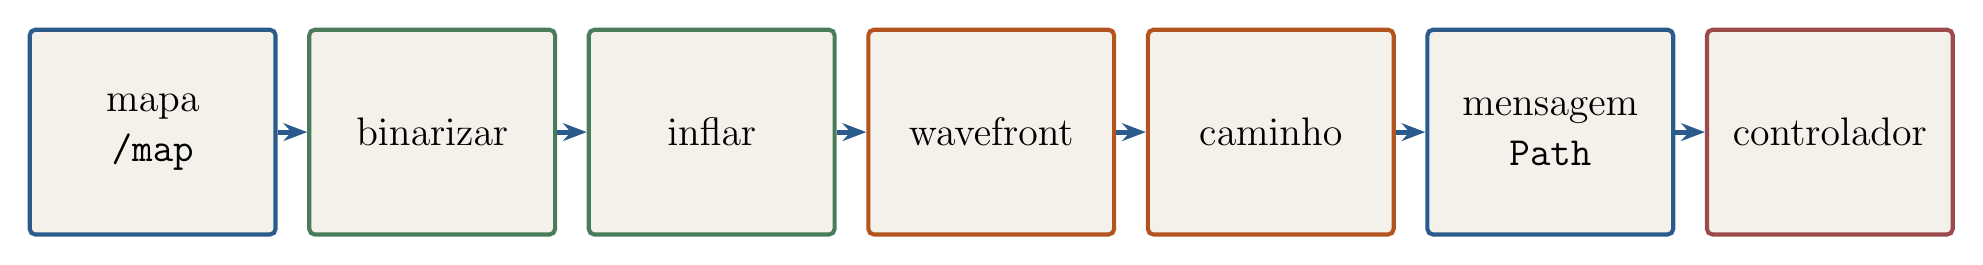
\begin{tikzpicture}[x=1cm,y=1cm]
\node[dbox, draw=dblue, line width=1.5pt, text width=2.7cm, minimum height=2.6cm, font=\Large] (b0) at (0.00,0) {mapa\\\texttt{/map}};
\node[dbox, draw=dgreen, line width=1.5pt, text width=2.7cm, minimum height=2.6cm, font=\Large] (b1) at (3.55,0) {binarizar};
\draw[dtrans, line width=1.8pt, -{Stealth[length=3mm]}] (b0.east) -- (b1.west);
\node[dbox, draw=dgreen, line width=1.5pt, text width=2.7cm, minimum height=2.6cm, font=\Large] (b2) at (7.10,0) {inflar};
\draw[dtrans, line width=1.8pt, -{Stealth[length=3mm]}] (b1.east) -- (b2.west);
\node[dbox, draw=dorange, line width=1.5pt, text width=2.7cm, minimum height=2.6cm, font=\Large] (b3) at (10.65,0) {wavefront};
\draw[dtrans, line width=1.8pt, -{Stealth[length=3mm]}] (b2.east) -- (b3.west);
\node[dbox, draw=dorange, line width=1.5pt, text width=2.7cm, minimum height=2.6cm, font=\Large] (b4) at (14.20,0) {caminho};
\draw[dtrans, line width=1.8pt, -{Stealth[length=3mm]}] (b3.east) -- (b4.west);
\node[dbox, draw=dblue, line width=1.5pt, text width=2.7cm, minimum height=2.6cm, font=\Large] (b5) at (17.75,0) {mensagem\\\texttt{Path}};
\draw[dtrans, line width=1.8pt, -{Stealth[length=3mm]}] (b4.east) -- (b5.west);
\node[dbox, draw=dred, line width=1.5pt, text width=2.7cm, minimum height=2.6cm, font=\Large] (b6) at (21.30,0) {controlador};
\draw[dtrans, line width=1.8pt, -{Stealth[length=3mm]}] (b5.east) -- (b6.west);
\end{tikzpicture}
\end{document}
